\documentclass[letterpaper, 11pt]{article}
\usepackage{comment} % enables the use of multi-line comments (\ifx \fi) 
\usepackage{fullpage} % changes the margin
\usepackage{fancyhdr} % for footer
\usepackage[UKenglish]{isodate}% http://ctan.org/pkg/isodate for date format
\usepackage{wrapfig}
\usepackage[font={small,sf}]{caption}
\usepackage{float}%force tables/figs into certain placement
\usepackage{graphicx}%for figures
\usepackage[leftcaption]{sidecap}%for figure captions
\usepackage{subcaption}%for figures
\usepackage{hyperref}%for hyperlinks
\usepackage[font=small,labelfont=bf]{caption}%for captions
%\usepackage{natbib}	%for bibliography
\usepackage{placeins}%prevent images from floating into inappropriate sections
\usepackage{tabulary}%for table at the end, to get soft wrapping
%\usepackage[capbesideposition=inside,facing=yes,capbesidesep=quad]{floatrow}
\usepackage[]{textcomp}%for degree symbol
\usepackage{titlesec}%to change appendix headers
\usepackage[titletoc,toc,title]{appendix}%to change appendix headers
\usepackage{gensymb}%for degree symbol

\usepackage{epigrafica}%changes default font to epigrafica
\usepackage[LGR,OT1]{fontenc}

\def\labelitemi{--}

\pagestyle{fancy}
\renewcommand{\headrulewidth}{0pt}

\lhead{}
\chead{}
\rhead{}
\lfoot{Frost Entomological Museum}
\cfoot{}
\rfoot{SOP 04 - \thepage}
\renewcommand{\footrulewidth}{0.4pt}
\title{SOP 04: Social Media}
\author{Frost Entomological Museum Curator \& Interest Group}
\DeclareTextAccent{\"}{OT1}{168}%adds diacritic

\begin{document}
\cleanlookdateon %removed ordinal date
\maketitle
\thispagestyle{fancy}

\section*{Preamble}
This SOP describes the strategies and etiquette relevant to the Frost Museum's social media presence.

\section{Etiquette}
All social media content must be \textit{relevant to entomology}, especially to ongoing activities at the Museum, and adhere to the social media guidelines established by Penn State and the College of Agricultural Sciences:
\begin{itemize}
\item \url{http://socialmedia.psu.edu/resources/} (PSU Social Media Hub)
\item \url{http://agsci.psu.edu/communications/how-to/social-media} (College social media guidelines)
\end{itemize}
Museum social media accounts must never be used to post material that is unlawful, obscene, abusive, defamatory, or which invades someone's privacy or publishes preliminary results without the researcher's permission. \\

\noindent{}Keep in mind that you are engaging the world through these resources---Facebook, Instagram, \textit{etc}.---as a representative of the Frost Entomological Museum and Penn State. Your goal should be to bring positive attention to the Museum and a greater awareness of the work that we do.

\section{Curators' blog}
\url{https://sites.psu.edu/frost/} \\

\noindent{}The Curators' blog should be updated at least weekly. Posts can be very short, highlighting a remarkable specimen, for example, to very long. All Museum employees are encourage to contribute content to the Curators' blog! And be sure to respond to comments. Contact the Director for access.

\subsection{Image use}

Ideally, each post should include at least one image, preferably produced in house. All images should be credited with the name of the photographer, licensing information, and a link to the source. \textit{Do not use copyrighted images}, unless you have the owner's permission in writing. 

\subsection{Mark-up best practices}

Users are encouraged to basic HTML, in order to produce robust content that is maximally accessible to readers of diverse abilities. Some tips for Museum bloggers:
\begin{itemize}
\item When you hyperlink some text be sure that it is relevant to the linked page and would be informative to an automated reader. Rather than linking multiple instances of the word ``here'' (You can find the original paper by Smith \underline{here}), for example, try linking to a string of words that describes what the link is for (The \underline{original paper by Smith} is available for download). 
\item Use the alt attribute when inserting an image. This mechanism gives you a chance to describe the image to a visually impaired person and to explain why it's relevant or funny (Figure \ref{altImage}).
\end{itemize}

\begin{figure}[ht!]
	\centering
  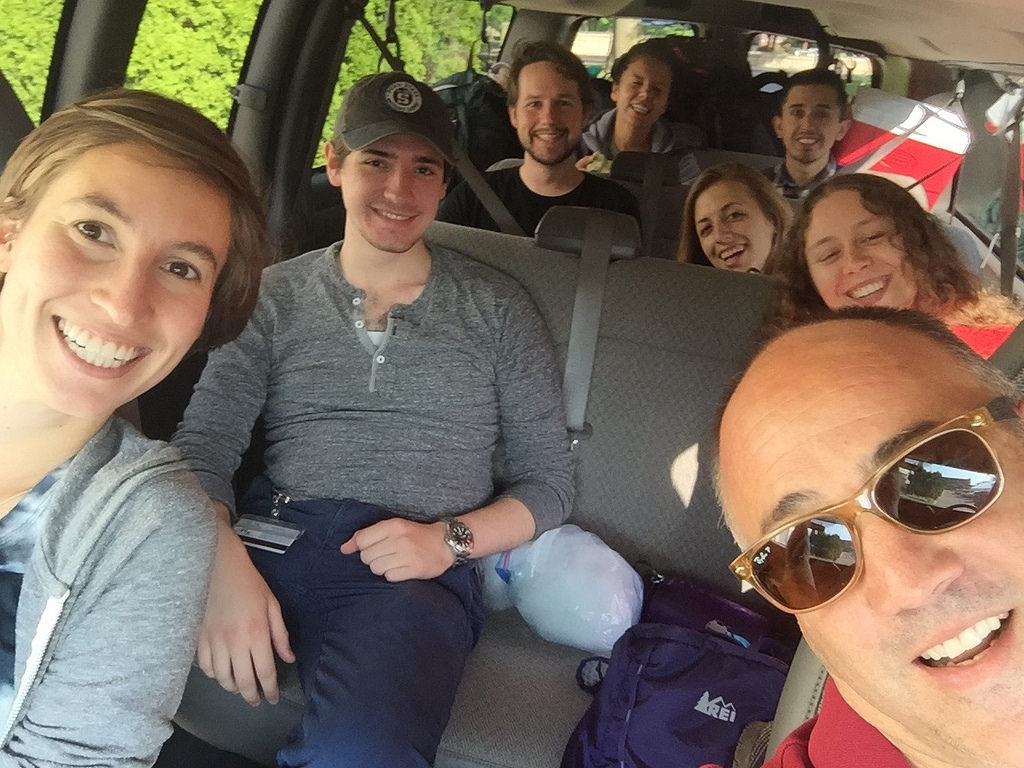
\includegraphics[width=0.55\textwidth]{dorksInAVan}
  \caption{From an actual post on the Curators' blog. The caption for this image reads ``Frost Museum cr\"ue, off to Philadelphia and then New Jersey Devil habitat''. Someone using an assisted Web browser might miss all the goofiness in the photo. We should attempt to make that aspect (the subtle jokes) accessible by using the alt attribute inside the img element: \hfill{}alt=``8 entomologists, looking like total nerds, smile for the camera phone while sitting in a van. The driver's neck looks like it's thicker than his head''}
  \label{altImage}
\end{figure}

\section{Flickr}
\url{https://flic.kr/ps/2qArpQ} \\

\noindent{}In order to make our photos and other images broadly available for reuse we deposit them on Flickr.com using a Creative Commons Attribution license (CC BY 2.0) and occasionally a public domain license (CC0). Note that licensing is governed the University and by our agreements with funding agencies (\textit{e.g.}, the National Science Foundation). Other flavors of the attribution license (CC BY 3.0, for example, or CC BY 4.0) are also acceptable. See Penn State's Copyright site for information: \url{http://copyright.psu.edu/creative-commons/}. Image metadata should also be relatively rich, so that we can trace photos back to specimens, taxa, photographer, etc.\\

\noindent{}For access to the Flickr account see the Director.

\section{Facebook}

\url{https://www.facebook.com/pages/Frost-Entomological-Museum/316418611712372}\\

\noindent{}The Museum's Facebook page primarily serves as a place to further distribute materials from other social media, for example blog posts. More information will likely go here when we are open to the public again.\\

\noindent{}Administrative access to the Facebook page is limited to the Director and Collection Manager. Please notify them of any problems.

\section{Twitter}
\url{https://twitter.com/FrostMuseum}\\

\noindent{}The Museum's Twitter feed primarily serves as a place to further distribute materials from other social media, for example blog posts. \\

\noindent{}Administrative access to the Twitter account is limited to the Director and Collection Manager. Please notify them of any problems.

\section{Instagram}
\url{https://www.instagram.com/frostentomologicalmuseum/}\\

The Museum's Instagram account highlights aspects of the collection and staff activities. All staff are encouraged to contribute images and videos.\\

\noindent{}For access to the Instagram account see the Director.

\section{Web site}
\url{http://ento.psu.edu/facilities/frost}\\

\noindent{}The official Frost Entomological Museum website is maintained by the Department as part of the College's broader website. Administrative access is limited to the Director and the Departmental webmaster.

%\clearpage
% adding bibliography here
%\bibliographystyle{unsrt}
%\bibliography{bib}

\end{document}


\\

\begin{figure}[ht!]
    \centering
    \begin{subfigure}[ht!]{0.43\textwidth}
        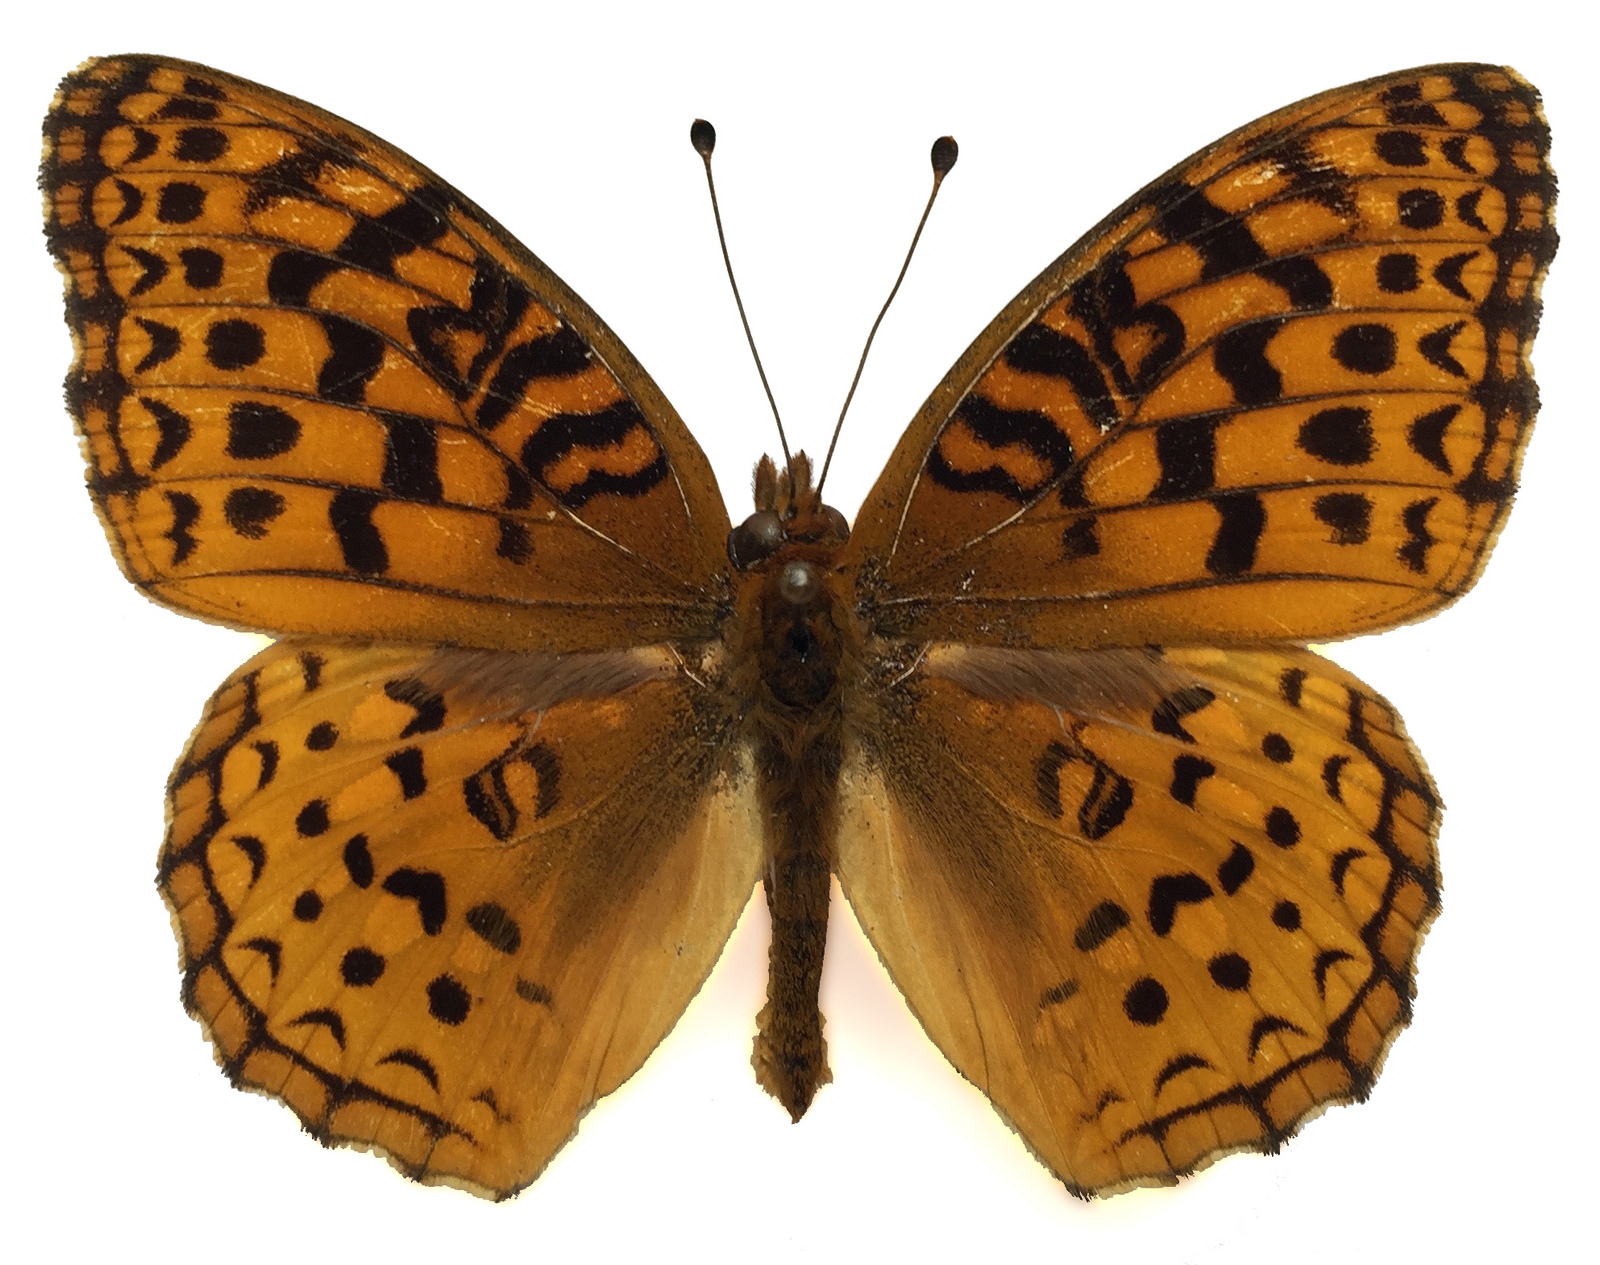
\includegraphics[width=\textwidth]{butterfly}
    \end{subfigure}
    \qquad
    \begin{subfigure}[ht!]{0.45\textwidth}
        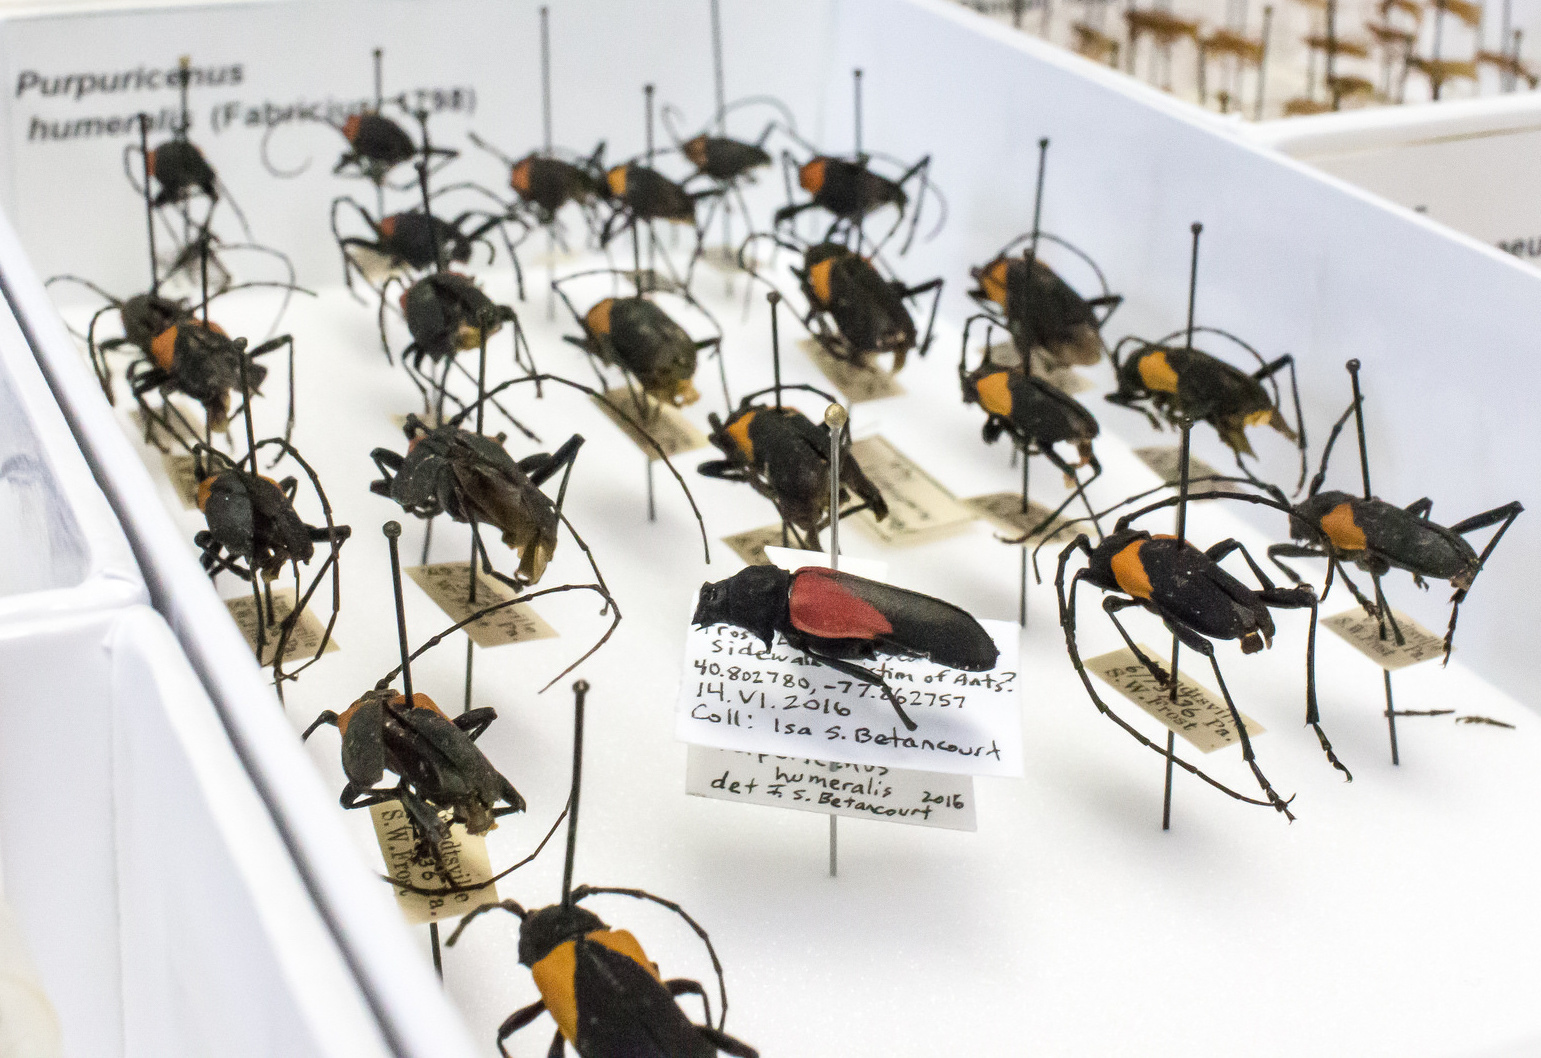
\includegraphics[width=\textwidth]{pinned}
    \end{subfigure}
    \caption{Frost Entomological Museum specimens. Photos CC BY 2.0 by Andy Deans (L) and Isa Betancourt (R)}
\end{figure}